\chapter{格点关联函数}

在第 4 节中,我们讨论了如何把 $\pi$介子的两点关联函数约化为夸克传播子(可能还包括规范链)的乘积,以及它与态求和之间的关系,从中可以提取出 $M_\pi$ 和 $f_\pi$。这里我把讨论推广到一般的两点与三点关联函数。考虑矩阵元 $\langle K^+|V_\mu|D^0\rangle$ 的计算,它出现在半轻子形状因子的提取中。计算这一矩阵元(ME)所需的三点关联函数为
\begin{equation}
\begin{aligned}
C_\mu^{PVP}(t_x, p; t_y, q) &=
\sum_{x,y} e^{-i(q\cdot y+p\cdot x)}\, T[K^+ V_\mu D^0] \\
&= \sum_{x,y} e^{-i(q\cdot y+p\cdot x)}\,
   \bar{s}(0)\gamma_5 u(0)\;\bar{c}(y)\gamma_\mu s(y)\;\bar{u}(x)\gamma_5 c(x) \\
&= \sum_{x,y} e^{-i(q\cdot y+p\cdot x)}\,
   \gamma_5 S_F^u(x,0)\gamma_5 S_F^s(0,y)\gamma_\mu S_F^u(y,x) \\
&\sim \frac{\exp(-E_K(p+q)t_y - E_D(p)(t_x-t_y))}{4E_K(p+q)E_D(p)}
   \langle 0|\bar{u}\gamma_5 s|K(p+q)\rangle \\
&\qquad \times \langle K(p+q)|\bar{s}\gamma_\mu c|D(p)\rangle
   \langle D(p)|\bar{c}\gamma_5 u|0\rangle .
\end{aligned}
\end{equation}

\begin{figure}[htbp]
\centering
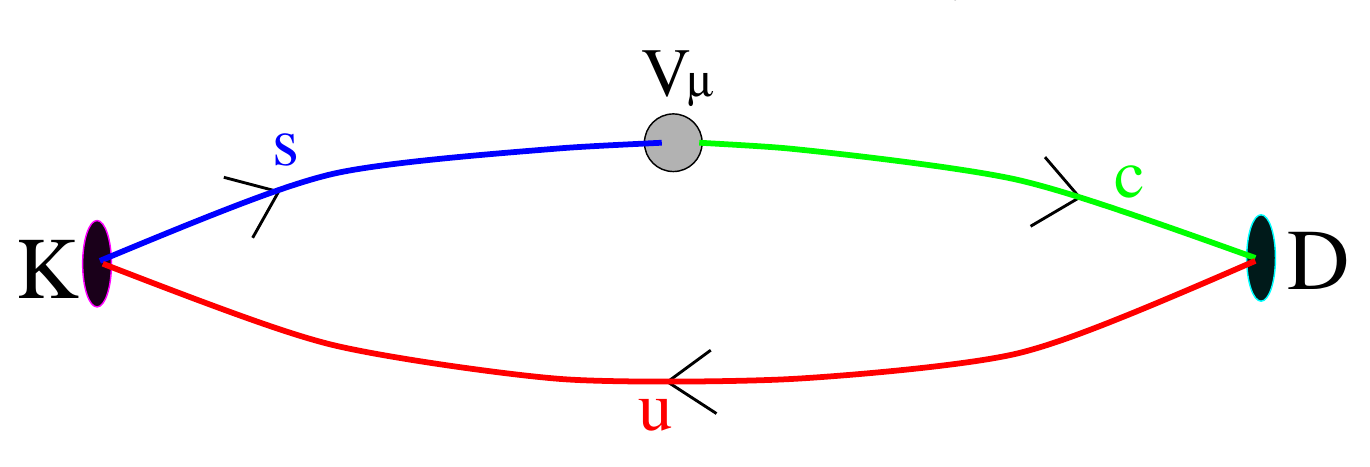
\includegraphics[width=0.8\textwidth]{images/fig20.png}
\caption{由 $c$、$s$ 和 $u$ 夸克传播子表示的 $KV_\mu D$ 费曼图示意。}
\label{fig:20}
\end{figure}

我用了 (i) Wick 收缩,把关联函数用夸克传播子 $S_F$ 表示出来(见图~20);(ii) 源与汇算符以及矢量流采用定域双线性(为了改善信号,通常使用涂抹算符和改进的流);(3) $D$ 介子的插值算符与流插入均具有确定的动量。于是动量守恒确定了 $p_k$。式~17.2 的最终形式给出了大欧几里得时间间隔($t_x \ll t_y \ll t_0$)下的行为。在右端的众多项中,我们只对矩阵元 $\langle K(p+q)|\bar{c}\gamma_\mu s|D(p)\rangle$ 感兴趣。其余因子都可以从两点关联函数中提取。因此,可以对所有需要的关联函数分别做拟合,或者设计一个比值,使尽可能多的不想要的因子相互抵消。实际上,为了改善数值信号,通常对三点关联函数与两点关联函数组合之比 $T[KV_\mu D]/(T[KK]\,T[DD])$ 做单个拟合,以消去随时间变化的指数行为。

为了对投影到确定空间动量上的这类关联函数做拟合,我们必须处理三个问题:
\begin{itemize}
\item 关联函数在其时间变量下是偶的还是奇的?
\item 关联函数在其动量下是偶的还是奇的?
\item 关联函数是实的还是虚的?如前所述,欧几里得关联函数只有实部有信号。
\end{itemize}

实际上,我们通常使用表~8 中给出的双线性算符,为简洁起见,其中 $i$ 的因子已被略去。在这一算符基下,需要知道给定的 $n$ 点函数是在实部还是虚部有信号。为了回答这些问题,我们利用表~2 与式~10.11 中讨论的离散对称性 $T$、$P$ 和 $CPH$。对于 Dirac 代数的每个元素 $\Gamma_A$,定义与 $T$、$P$ 和 $CPH$ 相关的三个符号 $\tau_A$、$\pi_A$ 和 $\chi_A$:
\begin{equation}
\begin{aligned}
\gamma_4\gamma_5\Gamma_A\gamma_5\gamma_4 &= \tau_A\Gamma_A;\\
\gamma_4\Gamma_A\gamma_4 &= \pi_A\Gamma_A;\\
C\gamma_4\gamma_5\Gamma_A\gamma_5\gamma_4 C^{-1} &= \chi_A\Gamma_A^* .
\end{aligned}
\end{equation}

\begin{table}[htbp]
\centering
\begin{tabular}{lcccccccc}
\toprule
 & $1$ & $\gamma_i$ & $\gamma_4$ & $\gamma_i\gamma_j$ & $\gamma_i\gamma_4$ & $\gamma_i\gamma_5$ & $\gamma_4\gamma_5$ & $\gamma_5$ \\
\midrule
$\tau_A$ & $+$ & $+$ & $-$ & $+$ & $-$ & $-$ & $+$ & $-$ \\
$\pi_A$ & $+$ & $-$ & $+$ & $+$ & $-$ & $+$ & $-$ & $-$ \\
$\chi_A$ & $+$ & $-$ & $+$ & $+$ & $-$ & $+$ & $-$ & $-$ \\
\bottomrule
\end{tabular}
\caption{双线性流在 $T$、$P$ 和 $CPH$ 变换下的符号。}
\label{tab:7}
\end{table}

这些符号列于表~7,其对两点与三点关联函数的应用将在下面两小节中说明。

\section{两点介子关联函数}

考虑一般的两点关联函数
\begin{equation}
\begin{aligned}
C^{BA}(p,t) &= \sum_x e^{-ip\cdot x}\,
   \langle \bar{\psi}_2(x)\Gamma_B\psi_1(x)\;\bar{\psi}_1(0)\Gamma_A\psi_2(0)\rangle ,\\
&= -\sum_x e^{-ip\cdot x}\,
   \mathrm{Tr}\big(S_2(0,x)\Gamma_B S_1(x,0)\Gamma_A\big) ,
\end{aligned}
\end{equation}

其中 Tr 表示对自旋和色指标求迹,$t \equiv x_4$。于是 $T$、$P$ 和 $CPH$ 蕴含如下结论:
\begin{itemize}
\item 若 $\tau_A\tau_B = \pm 1$,$C^{BA}(p,t)$ 关于 $t$ 为偶(奇)。
\item 若 $\pi_A\pi_B = \pm 1$,$C^{BA}(p,t)$ 关于 $p$ 为偶(奇)。
\item 若 $\chi_A\chi_B = \pm 1$,$C^{BA}(p,t)$ 为实(虚)。
\end{itemize}

注意在式~17.3 中,第二个夸克传播子是从 $x \to 0$。利用厄米性性质 $S(x,0) = \gamma_5 S(0,x)^\dagger \gamma_5$,我们可将其用 $S(x,0)$ 表示。这一简单性质——从某一点出发的夸克传播子与到达该点的反夸克传播子之间的关系——带来巨大的计算节省。例如,若动量投影通过对 $L^3$ 个汇点 $x$ 以权重 $\exp(ip\cdot x)$ 求和来完成,那么由于厄米性性质,我们只需一次传播子求逆,而不是 $L^3+1$ 次。

\section{插值算符}

对于类威尔逊费米子,零动量下介子和重子的插值场算符列于表~8。为简洁起见,三种味标记为 $u$、$d$、$s$。重子算符需要进一步说明,如文献 [156] 所讨论,现复述如下。

\begin{table}[htbp]
\centering
\begin{tabular}{lll}
\toprule
态 & $I^G(J^{PC})$ & 算符 \\
\midrule
标量($\sigma$) & $1^-(0^{++})$ & $u(x)d(x)$ \\
                  & $1^-(0^{++})$ & $u(x)\gamma_4 d(x)$ \\
赝标量      & $1^-(0^{-+})$ & $u(x)\gamma_5 d(x)$ \\
                  & $1^-(0^{-+})$ & $u(x)\gamma_4\gamma_5 d(x)$ \\
矢量            & $1^+(1^{--})$ & $u(x)\gamma_i d(x)$ \\
                  & $1^+(1^{--})$ & $u(x)\gamma_i\gamma_4 d(x)$ \\
轴矢($a_1$)     & $1^-(1^{++})$ & $u(x)\gamma_i\gamma_5 d(x)$ \\
张量($b_1$)    & $1^+(1^{+-})$ & $u(x)\gamma_i\gamma_j d(x)$ \\
\midrule
核子八重态     & $(\tfrac{1}{2},\tfrac{1}{2}^-)$ & $(u_a^T C d_b)\,\gamma_5 s_c\,\epsilon_{abc}$ \\
                  & $(\tfrac{1}{2},\tfrac{1}{2}^-)$ & $(u_a^T C\gamma_5 d_b)\,s_c\,\epsilon_{abc}$ \\
Delta 十重态    & $(\tfrac{3}{2},\tfrac{3}{2}^+)$ & $(u_a^T C\gamma_i d_b)\,s_c\,\epsilon_{abc}$ \\
\bottomrule
\end{tabular}
\caption{类威尔逊理论中介子和重子的定域插值场算符。通过对时间片上各点 $x$ 求和即得到向零动量态的投影。$C$ 字称只对味简并的介子态有意义。重子算符中的 $(\ )$ 表示自旋求迹。$C = \gamma_2\gamma_4$,核子味指标的对称性质在正文中讨论。十重态重子算符在味指标下完全对称。}
\label{tab:8}
\end{table}

自旋 1/2 的重子由下列插值算符产生
\begin{equation}
O_{(ij)k} = (\psi_{a,i}^T C\gamma_5 \psi_{b,j})\,\psi_{c,k}\,\epsilon_{abc} ,
\end{equation}

其中 $a$、$b$ 和 $c$ 标记色指标,而 $i$、$j$ 和 $k$ 标记味指标。容易证明 $O_{(ij)k} = -O_{(ji)k}$,因此只有九个独立的算符——八个 $SU(3)$ 八重态以及单态 $\sum_{ijk}\epsilon_{ijk}O_{ijk}$。投影掉单态的一种方法是构造
\begin{equation}
B_{ijk} = O_{(ij)k} + O_{(ik)j} = B_{ikj} .
\end{equation}

有八个独立的 $B_{ijk}$,它们与通常态之间的关系由下例说明
\begin{equation}
\begin{aligned}
\sqrt{2}\,p &= -B_{duu} = 2B_{uud} = 2B_{udu},\\
\sqrt{2}\,\Sigma^+ &= -B_{suu} = 2B_{uus} = 2B_{usu},\\
\Sigma^0 &= B_{uds} + B_{dsu} = -B_{sud},\\
\sqrt{3}\,\Lambda^0 &= B_{uds} - B_{dsu}.
\end{aligned}
\end{equation}

这些方程中的总体因子是任意的,而相对归一化由 $SU(3)$ 对称性确定。所有自旋 1/2 重子关联函数都由图~21 所示的两种收缩构成。记号 $\langle DU\rangle_S = \langle UD\rangle_S$ 对应味为 $U$ 和 $D$ 的夸克收缩成一个闭合圈,而 $S$ 的传播子携带重子的自旋量子数。记号 $(DUS)$ 对应三个夸克的一种有序收缩。我们考虑两种类型的关联函数,即「$\Sigma$ 型」和「$\Lambda$ 型」。前者以 $\Sigma^0$ 为例

\begin{figure}[htbp]
\centering
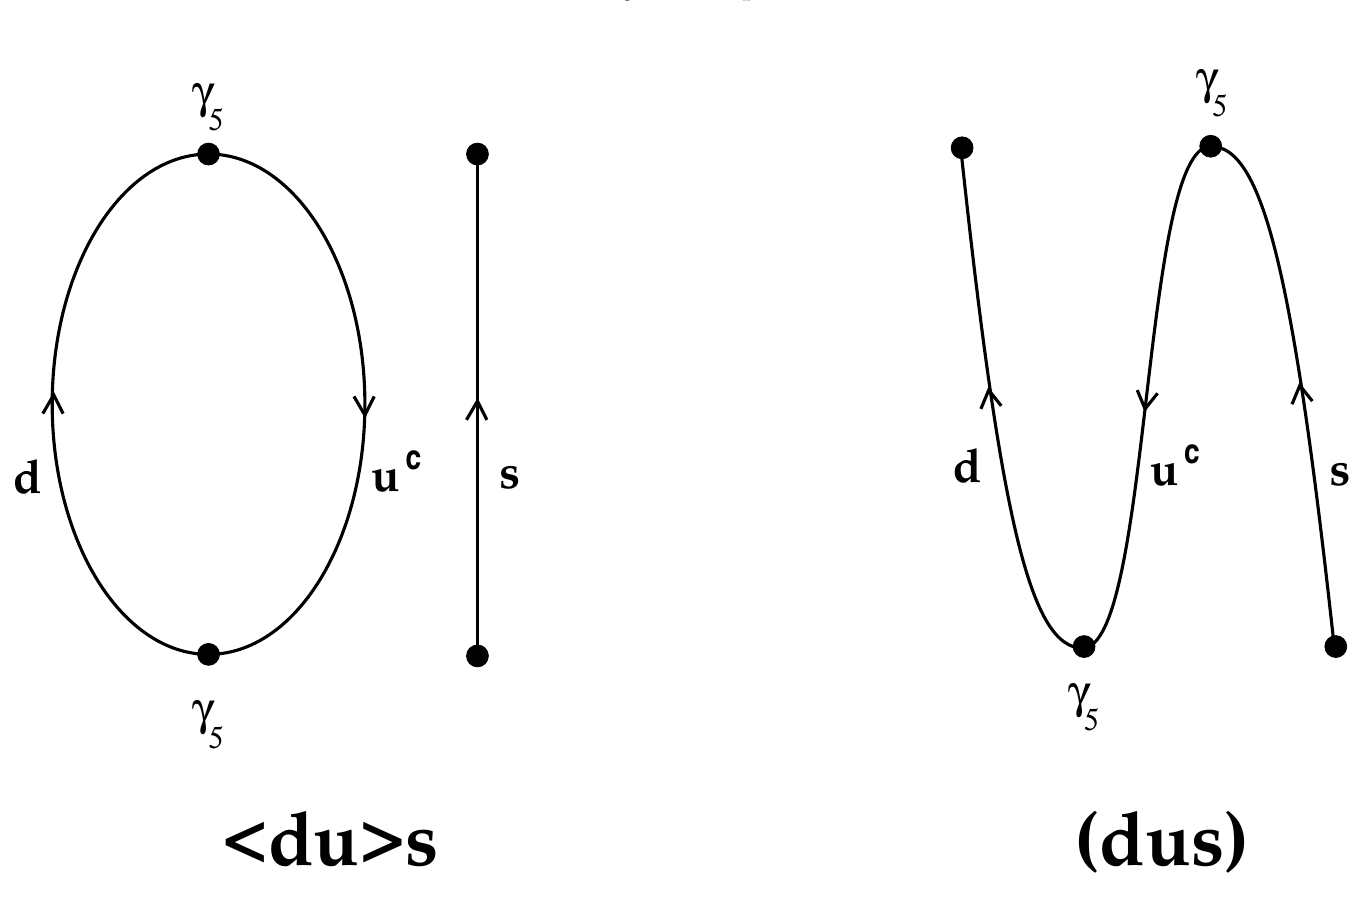
\includegraphics[width=0.8\textwidth]{images/fig21.png}
\caption{重子态的两种不同类型的收缩。}
\label{fig:21}
\end{figure}

\begin{equation}
S_{\{UD\}} = S_{\{DU\}} \equiv \langle B_{sud}(x)B_{sud}(0)\rangle
= \langle US\rangle_D + \langle DS\rangle_U + (USD) + (DSU) .
\end{equation}

此方程定义了收缩的符号约定。质子、中子、$\Sigma^+$、$\Sigma^-$、$\Xi^0$ 和 $\Xi^-$ 的关联函数也属于这种类型:它们分别是 $D\{UU\}$、$U\{DD\}$、$S\{UU\}$、$S\{DD\}$、$U\{SS\}$ 和 $D\{SS\}$。第二种类型的关联函数是 $\Lambda^0$ 的
\begin{equation}
\begin{split}
S_{[UD]} = S_{[DU]} &\equiv \tfrac{1}{3}\Big[\langle US\rangle_D + \langle DS\rangle_U + 4\langle UD\rangle_S\\
&\qquad - (USD) - (DSU) + 2(SUD) + 2(SDU) + 2(UDS) + 2(DUS)\Big] .
\end{split}
\end{equation}

当 $m_u \neq m_d$ 时,还存在一个非零的 $\Lambda^0 - \Sigma^0$ 交叉关联函数,但尚未找到有用的结果 [156]。形如 $A[AB]$ 和 $A\{AB\}$ 的关联函数不是独立的——它们由下式联系
\begin{equation}
\begin{aligned}
A_{[AB]} &= \tfrac{1}{4}(3B_{[AA]} + B_{\{AA\}}),\\
A_{\{AB\}} &= \tfrac{1}{4}(B_{[AA]} + 3B_{\{AA\}}) .
\end{aligned}
\end{equation}

可以把 $A\{BB\}$ 和 $A[BB]$ 的质量结果分别视为 $\Sigma$ 和 $\Lambda$ 在 $m_s = m_A$、$m_u = m_d = m_B$ 情形下的结果。与真实世界不同,这里没有任何东西阻止 $m_A = m_B$。但请注意,在这种情况下 $\Sigma$ 和 $\Lambda$ 也是简并的,即 $M(A\{AA\}) = M(A[AA])$。事实上,两种情形下的收缩完全相同。

完全非简并关联函数 $A[BC]$ 和 $A\{BC\}$ 结果的解释更为复杂。由于同位旋被破坏,$\Sigma^0$ 型和 $\Lambda$ 型态会发生混合,两个关联函数都包含来自两个物理态的贡献。设 $M_+$ 和 $M_-$ 分别为较重和较轻态的质量,$\delta M$ 为质量差。在长时间下,两个关联函数的有效质量都将渐近到 $M_-$。然而,在与质量差的倒数相比很短的时间下,即 $\delta M\,t_{\max} \ll 1$,会有一个近似平台,其值是两个质量的加权平均。文献 [156] 在手征展开的最低阶导出的令人惊讶的结果是,从这些短时平台提取的质量对同位旋破缺不敏感,可以解释为 $A[DD]$ 和 $A\{DD\}$ 的质量,其中 $D = (B+C)/2$ 是两个夸克的平均质量。

\section{三点关联函数}

由介子算符和双线性流构成的一般三点关联函数具有如下形式
\begin{equation}
\begin{aligned}
C^{CBA}(q,t_y;p,t_x) &= \sum_{x,y} e^{-i(q\cdot y+p\cdot x)}\,
   \langle \bar{\psi}_3(y)\Gamma_C\psi_2(y)\;\bar{\psi}_2(x)\Gamma_B\psi_1(x)
   \;\bar{\psi}_1(0)\Gamma_A\psi_3(0)\rangle ,\\
&= -\sum_{x,y} e^{-i(q\cdot y+p\cdot x)}\,
   \mathrm{Tr}\big(S_3(0,y)\Gamma_C S_2(y,x)\Gamma_B S_1(x,0)\Gamma_A\big) ,
\end{aligned}
\end{equation}

其中 $t_x \equiv x_4$ 和 $t_y \equiv y_4$。$T$、$P$ 和 $CPH$ 蕴含
\begin{itemize}
\item 若 $\tau_A\tau_B\tau_C = \pm 1$,$C^{CBA}(q,t_y;p,t_x)$ 在 $t_x$ 和 $t_y$ 同时反号下为偶(奇)。
\item 若 $\pi_A\pi_B\pi_C = \pm 1$,$C^{CBA}(q,t_y;p,t_x)$ 在 $p$ 和 $q$ 同时反号下为偶(奇)。
\item 若 $\chi_A\chi_B\chi_C = \pm 1$,$C^{CBA}(q,t_y;p,t_x)$ 为实(虚)。
\end{itemize}

\section{CPS 对称性}

该理论还有一个附加的离散对称性 $CPS$,其中 $S$ 是交换 $s$ 夸克和 $d$ 夸克之间的对称性 [157]。当 $m_d = m_s$ 时,这一对称性在格点和连续中都成立。当 $m_d \neq m_s$ 时,对称性被软破缺,即破缺量与 $m_s - m_d$ 成正比。这一对称性在弱矩阵元的计算中起着非常重要的作用,因为它 (i) 限制了可能的 Wick 收缩的集合,(ii) 限制了相互混合的算符集合。

举一个简单的例子,考虑 $(\bar{s}\gamma_\mu Lu)(\bar{u}\gamma_\mu Ld)$,这是一个在 $CPS$ 下为偶的定域四夸克算符
\begin{equation}
\begin{aligned}
(\bar{s}\gamma_\mu Lu)(\bar{u}\gamma_\mu Ld)
&\xrightarrow{P} (\bar{s}\gamma_4\gamma_\mu L\gamma_4 u)(\bar{u}\gamma_4\gamma_\mu L\gamma_4 d)\\
&\xrightarrow{C} (s^T C^{-1}\gamma_4\gamma_\mu L\gamma_4 C\bar{u}^T)(u^T C^{-1}\gamma_4\gamma_\mu L\gamma_4 C\bar{d}^T)\\
&= (s^T\gamma_4\gamma_\mu^T L\gamma_4\bar{u}^T)(u^T\gamma_4\gamma_\mu^T L\gamma_4\bar{d}^T)\\
&= (s^T\gamma_\mu^T R\bar{u}^T)(u^T\gamma_\mu^T R\bar{d}^T)\\
&= (\bar{u}R\gamma_\mu s)(\bar{d}R\gamma_\mu u)\\
&= (\bar{u}\gamma_\mu Ls)(\bar{d}\gamma_\mu Lu)\\
&\xrightarrow{S} (\bar{u}\gamma_\mu Ld)(\bar{s}\gamma_\mu Lu)
\end{aligned}
\end{equation}

括号表示对自旋和色求迹,最后对两个求迹项的重新排序是允许的,因为在计算期望值时隐含了时间排序。

正如 Bernard 和 Soni 在文献 [2,6] 中所讨论的,这一对称性还有进一步的推广。对于形如 $(\bar{\psi}_1\Gamma_A\psi_2)(\bar{\psi}_3\Gamma_B\psi_4)$ 的四费米子算符,有两种一般的交换:(i) $CPS'$,对应 $1 \leftrightarrow 2$ 和 $3 \leftrightarrow 4$;(ii) $CPS''$,对应 $1 \leftrightarrow 4$ 和 $2 \leftrightarrow 3$。Bernard 和 Soni 在 [2,6] 中展示了如何利用这些交换对称性来限制 (i) 通过算符 $(\bar{s}\gamma_\mu Lu)(\bar{u}\gamma_\mu Ld)$ 在衰变 $K \to \pi\pi$ 中可能的收缩,以及 (ii) $O_\pm \equiv (\bar{s}\gamma_\mu Ld)(\bar{u}\gamma_\mu Lu) \pm (\bar{s}\gamma_\mu Lu)(\bar{u}\gamma_\mu Ld) - (u \to c)$ 与其他算符的混合。我把这些计算的细节留作读者的练习。
